\section{Method} \label{sec: method}


\subsection{Overall Encoding Framework} \label{sec: overall encoding framework}

\begin{figure}[t]
	\centering
	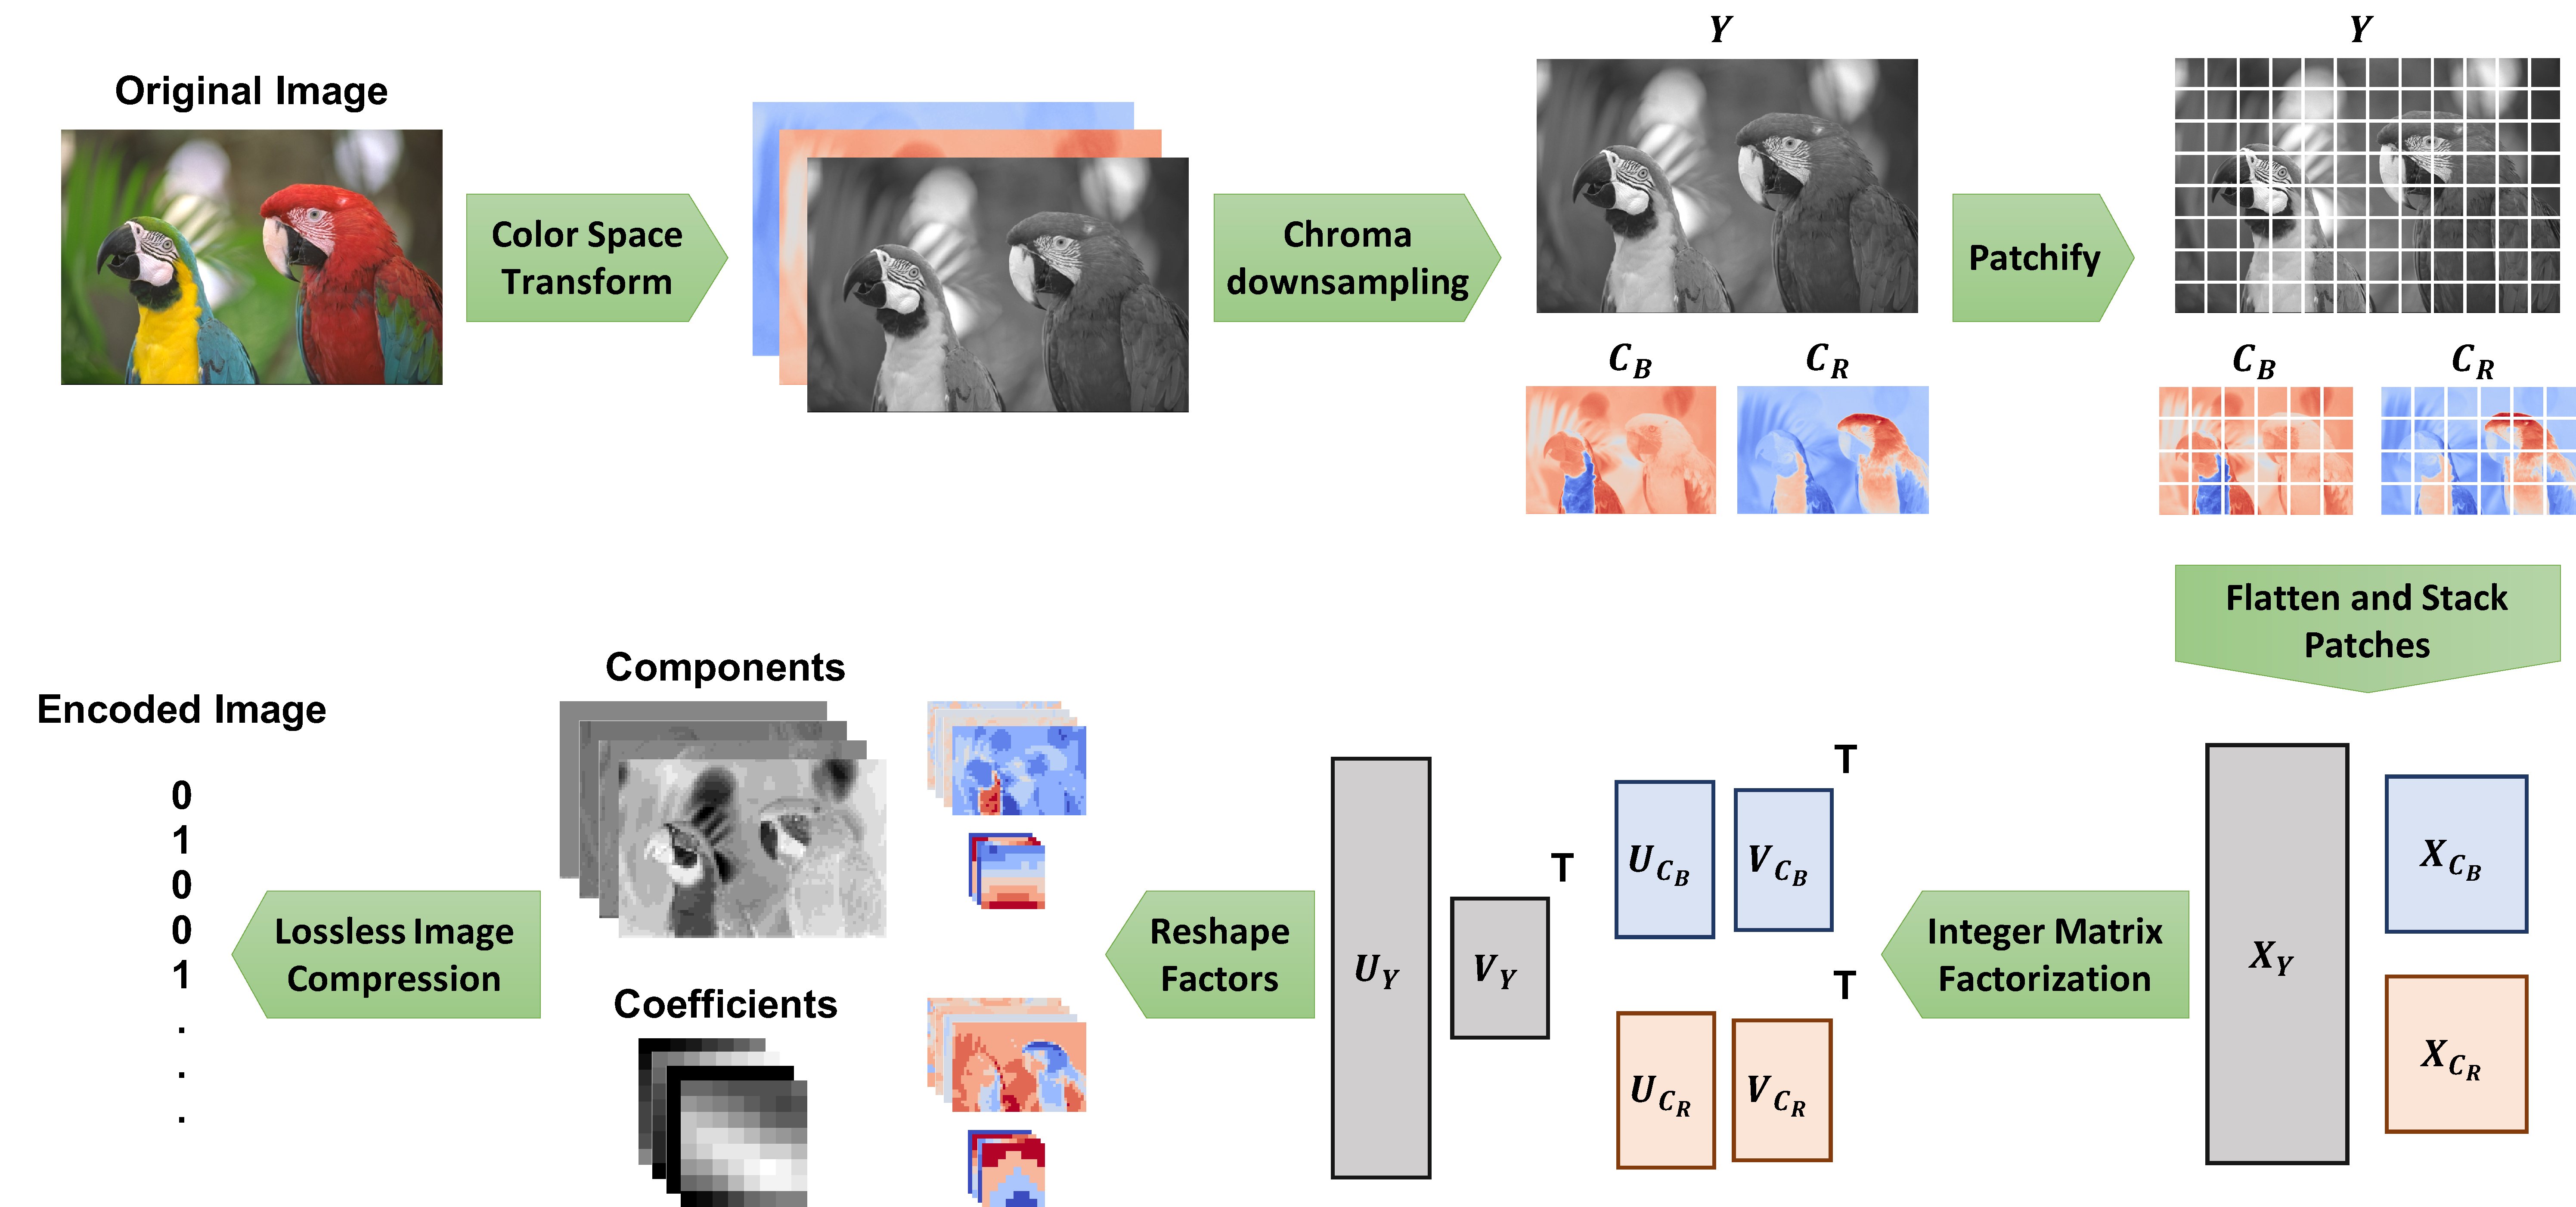
\includegraphics[width=\linewidth]{figures/imf_encoder.pdf}
	\vspace{10pt}
	\caption{An illustration of the encoder for our image compression method, based on integer matrix factorization.}
	\label{fig:imf_encoder}
\end{figure}

Figure \ref{fig:imf_encoder} illustrates an overview of the encoding pipeline for our proposed image compression method using integer matrix factorization (IMF). The encoder accepts an RGB image with dimensions $H \times W$ and a color depth of 8 bits, represented by the tensor $\bm{\mathcal{X}} \in \{0, \ldots, 255\}^{3 \times H \times W}$. Each step of encoding is described in the following.

\paragraph{Color Space Transformation.}
Analogous to the JPEG standard, the image is initially transformed into the YC\textsubscript{B}C\textsubscript{R} color space. Let $\bm{Y} \in [0, 255]^{H \times W}$ represent the \emph{luma} component, and $\bm{C}_B, \bm{C}_R \in [0, 255]^{\frac{H}{2} \times \frac{W}{2}}$ represent the blue-difference and red-difference \emph{chroma} components, respectively. Note that as a result of this transformation, the elements of the \emph{luma} ($\bm{Y}$) and \emph{chroma} ($\bm{C}_B$, $\bm{C}_R$) matrices are not limited to integers and can take any value within the interval $[0, 255]$.

\paragraph{Chroma Downsampling.} 
After conversion to the YC\textsubscript{B}C\textsubscript{R} color space, the \emph{chroma} components $\bm{C}_B$ and $\bm{C}_R$ are downsampled using average-pooling with a kernel size of $(2, 2)$ and a stride of $(2, 2)$, similar to the process used in JPEG. This downsampling exploits the fact that the human visual system perceives far more detail in brightness information (\emph{luma}) than in color saturation (\emph{chroma}).

\paragraph{Patchification.}
After \emph{chroma} downsampling, we have three components:  the \emph{luma} component $\bm{Y} \in [0, 255]^{H \times W}$ and the \emph{chroma} components $\bm{C}_B, \bm{C}_R \in [0, 255]^{\frac{H}{2} \times \frac{W}{2}}$. Each of the matrices is split into non-overlapping $8 \times 8$ patches. If a dimension of a matrix is not divisible by 8, the matrix is first padded to the nearest size divisible by 8 using reflection of the boundary values. These patches are then flattened into row vectors and stacked vertically to form matrices $\bm{X}_{Y} \in [0, 255]^{\frac{HW}{64} \times 64}$, $\bm{X}_{C_B} \in [0, 255]^{\frac{HW}{256} \times 64}$, and $\bm{X}_{C_R} \in [0, 255]^{\frac{HW}{256} \times 64}$. Later, these matrices will be low-rank approximated using integer matrix factorization (IMF). Note that this patchification technique differs from the block splitting in JPEG, where each block is subject to discrete cosine transform (DCT) and processed independently. This patchification technique not only captures the locality and spatial dependencies of neighboring pixels \doublecheck{but also performs better with the matrix decomposition approach to image compression. $\gets$ rephrase the sentence.}

\paragraph{Low-rank approximation.} 
We now apply a low-rank approximation to the matrices $\bm{X}_{Y}$, $\bm{X}_{C_B}$, and $\bm{X}_{C_R}$, which is the core of our compression method that provides a lossy compressed representation of these matrices.  The low-rank approximation \citep{eckart1936approximation} aims to approximate a given matrix $ \bm{X} \in \mathbb{R}^{M \times N} $ by 
\begin{equation} \label{eq: lra}
	\bm{X} \approx \bm{U} \bm{V}^\mathsf{T} = \sum_{r=1}^{R} U_{:r} {V_{:r}}^\mathsf{T},
\end{equation} 
where $\bm{U} \in \mathbb{R}^{M \times R}$ and $\bm{V} \in \mathbb{R}^{N \times R}$ are \emph{factor matrices} (or simply \emph{factors}), $R \leq \min(M,N)$ represents the \emph{rank}, $U_{:r}$ and $V_{:r}$ represent the $r$-th columns of $\bm{U}$ and $\bm{V}$, respectively. We refer to $\bm{U}$ as the \emph{basis matrix} and $\bm{V}$ as the \emph{coefficient matrix}. By selecting a sufficiently small value for $R$, the factor matrices $\bm{U}$ and $\bm{V}$, with a combined total of $(M+N)R$ elements, offer a compact representation of the original matrix $\bm{X}$, which has $MN$ elements, capturing the most significant patterns in the image. Depending on the loss function used to measure the reconstruction error between $\bm{X}$ and the product $\bm{U} \bm{V}^\mathsf{T}$, as well as the constraints on the factor matrices $\bm{U}$ and $\bm{V}$, various formulations and variants have been proposed for different purposes \doublecheck{$\gets$ make sure you cite some works here and/or in the intro}. In Section \ref{sec: imf}, we introduce and elaborate on our variant, termed integer matrix factorization (IMF), and argue why it is well-suited and effective for image compression. 

\paragraph{Reshape factors.} 
IMF yields integers factor matrices $\bm{U}_{Y} \in \{0, \ldots, 255\}^{\frac{HW}{64} \times R}$ and $\bm{V}_{Y} \in \{0, \ldots, 255\}^{64 \times R}$; $\bm{U}_{C_B} \in \{0, \ldots, 255\}^{\frac{HW}{256} \times R}$ and $\bm{V}_{C_B} \in \{0, \ldots, 255\}^{64 \times R}$; and $\bm{U}_{C_R} \in \{0, \ldots, 255\}^{\frac{HW}{256} \times R}$ and $\bm{V}_{C_R} \in \{0, \ldots, 255\}^{64 \times R}$ that correspond to $\bm{X}_{Y}$, $\bm{X}_{C_B}$, and $\bm{X}_{C_R}$. We reshape these matrices by unfolding their first dimension to obtain $R$-channel 2D spatial maps, referred to as \emph{factor maps} and represented by the following tensors:
\begin{align} \label{eq: reshaped factors}
	\bm{\mathcal{U}}_{Y} & \in \{0, \ldots, 255\}^{R \times \frac{H}{8} \times \frac{W}{8}}, \nonumber \\
	\bm{\mathcal{U}}_{C_B}, \bm{\mathcal{U}}_{C_R} & \in \{0, \ldots, 255\}^{R \times \frac{H}{16} \times \frac{W}{16}}, \\
	\bm{\mathcal{V}}_{Y}, \bm{\mathcal{V}}_{C_B}, \bm{\mathcal{V}}_{C_R} & \in \{0, \ldots, 255\}^{R \times 8 \times 8}. \nonumber
\end{align}

\paragraph{Lossless image compression.}
Since \emph{factor maps} are already integer tensors, we do not need a quantization step, which is commonly present in other lossy image compression methods and adds extra complications. This is the main advantage of our approach. Moreover, each channel of a \emph{factor map} can be treated as an 8-bit grayscale image and therefore can be directly encoded by any standard lossless image compression method, such as PNG or WebP. For images with a resolution of $H, W \gg 64$, which are most common nowadays, the basis maps ($\bm{\mathcal{U}}$) are significantly larger than the coefficient maps ($\bm{\mathcal{V}}$), accounting for the majority of the storage space. Interestingly, in practice, the IMF basis maps turn out to be meaningful images, each capturing some visual semantic of the image (see Figure \ref{fig:imf_components} for an example). Therefore, our IMF approach can effectively leverage the power of existing lossless image compression algorithms, offering a significant advantage over current methods.

\begin{figure}[t]
    \centering
    \begin{minipage}{0.41\textwidth}
        \begin{subfigure}{\textwidth}
            \centering
            \includegraphics[width=.95\textwidth]{figures/kodim23_Y_components.pdf}
            \vspace{-13pt}
            \caption{$\bm{\mathcal{U}}_Y$ channels}
        \end{subfigure}%
    \end{minipage}
    \hspace{0.1cm} 
    \begin{minipage}{0.35\textwidth}
        \centering
        \begin{minipage}{\textwidth}
            \begin{subfigure}{\textwidth}
                \centering
                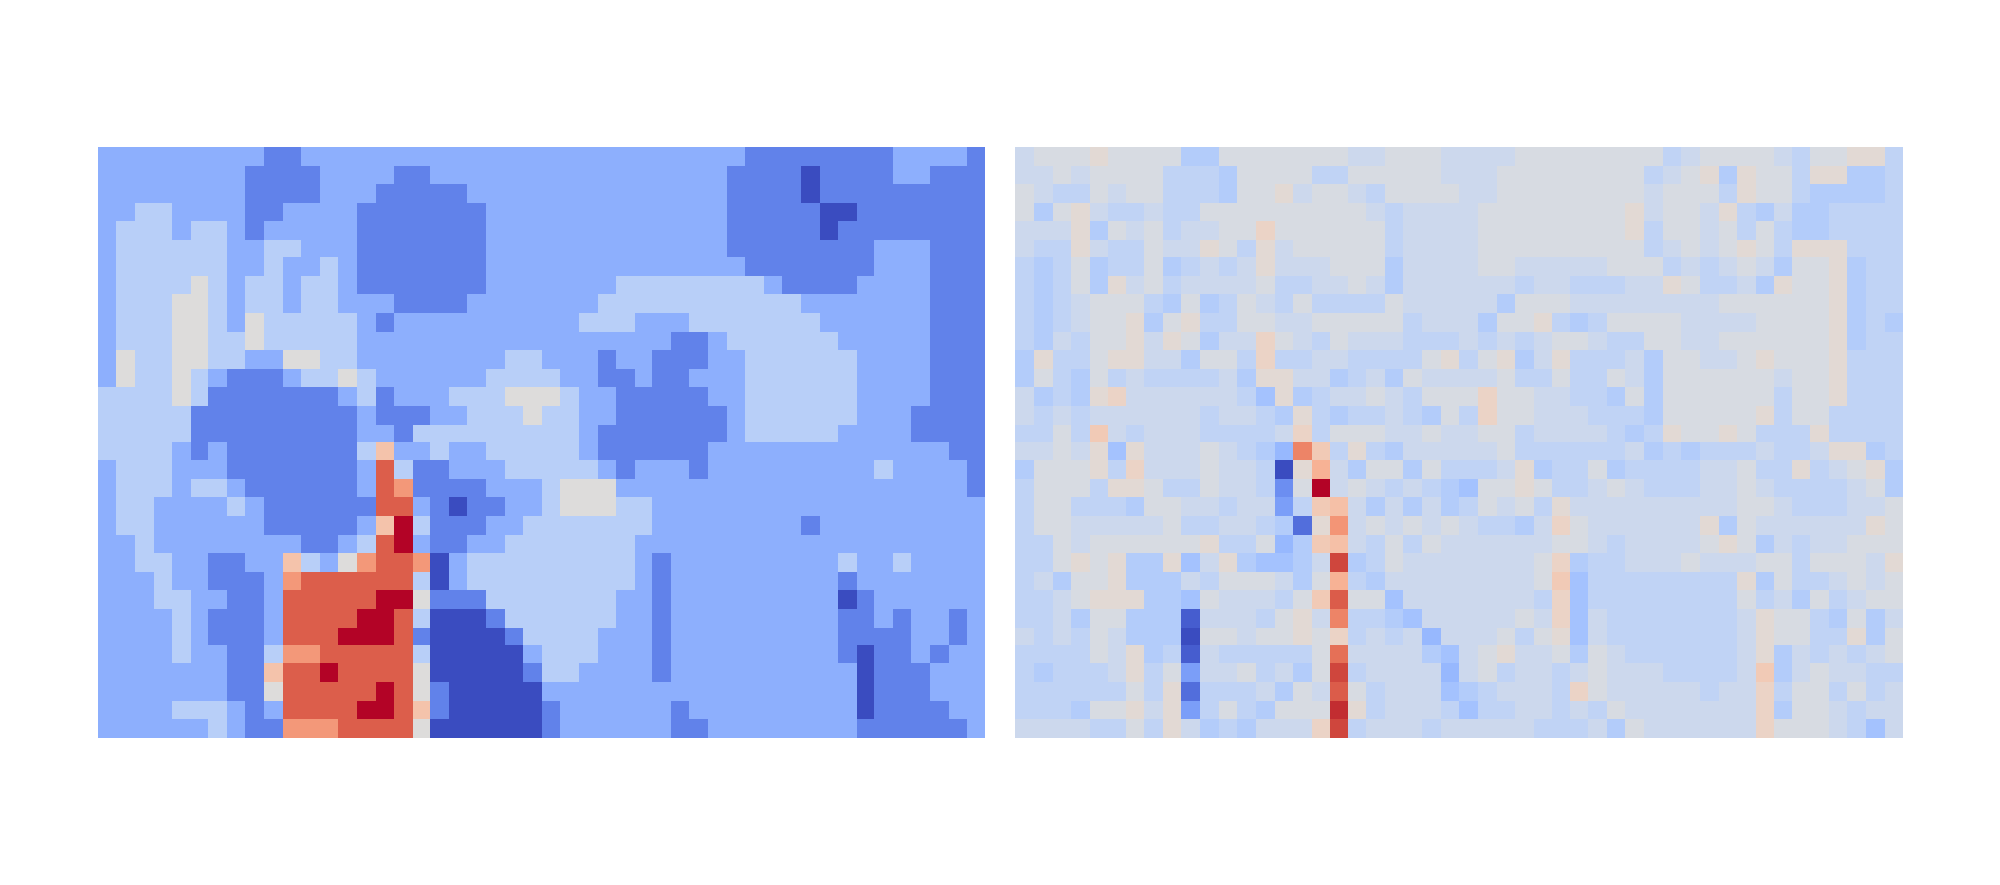
\includegraphics[width=.95\textwidth]{figures/kodim23_cb_components.pdf}
                \vspace{-15pt}
                \caption{$\bm{\mathcal{U}}_{C_B}$ channels}
            \end{subfigure}%
        \end{minipage}
        \begin{minipage}{\textwidth}
            \begin{subfigure}{\textwidth}
                \centering
                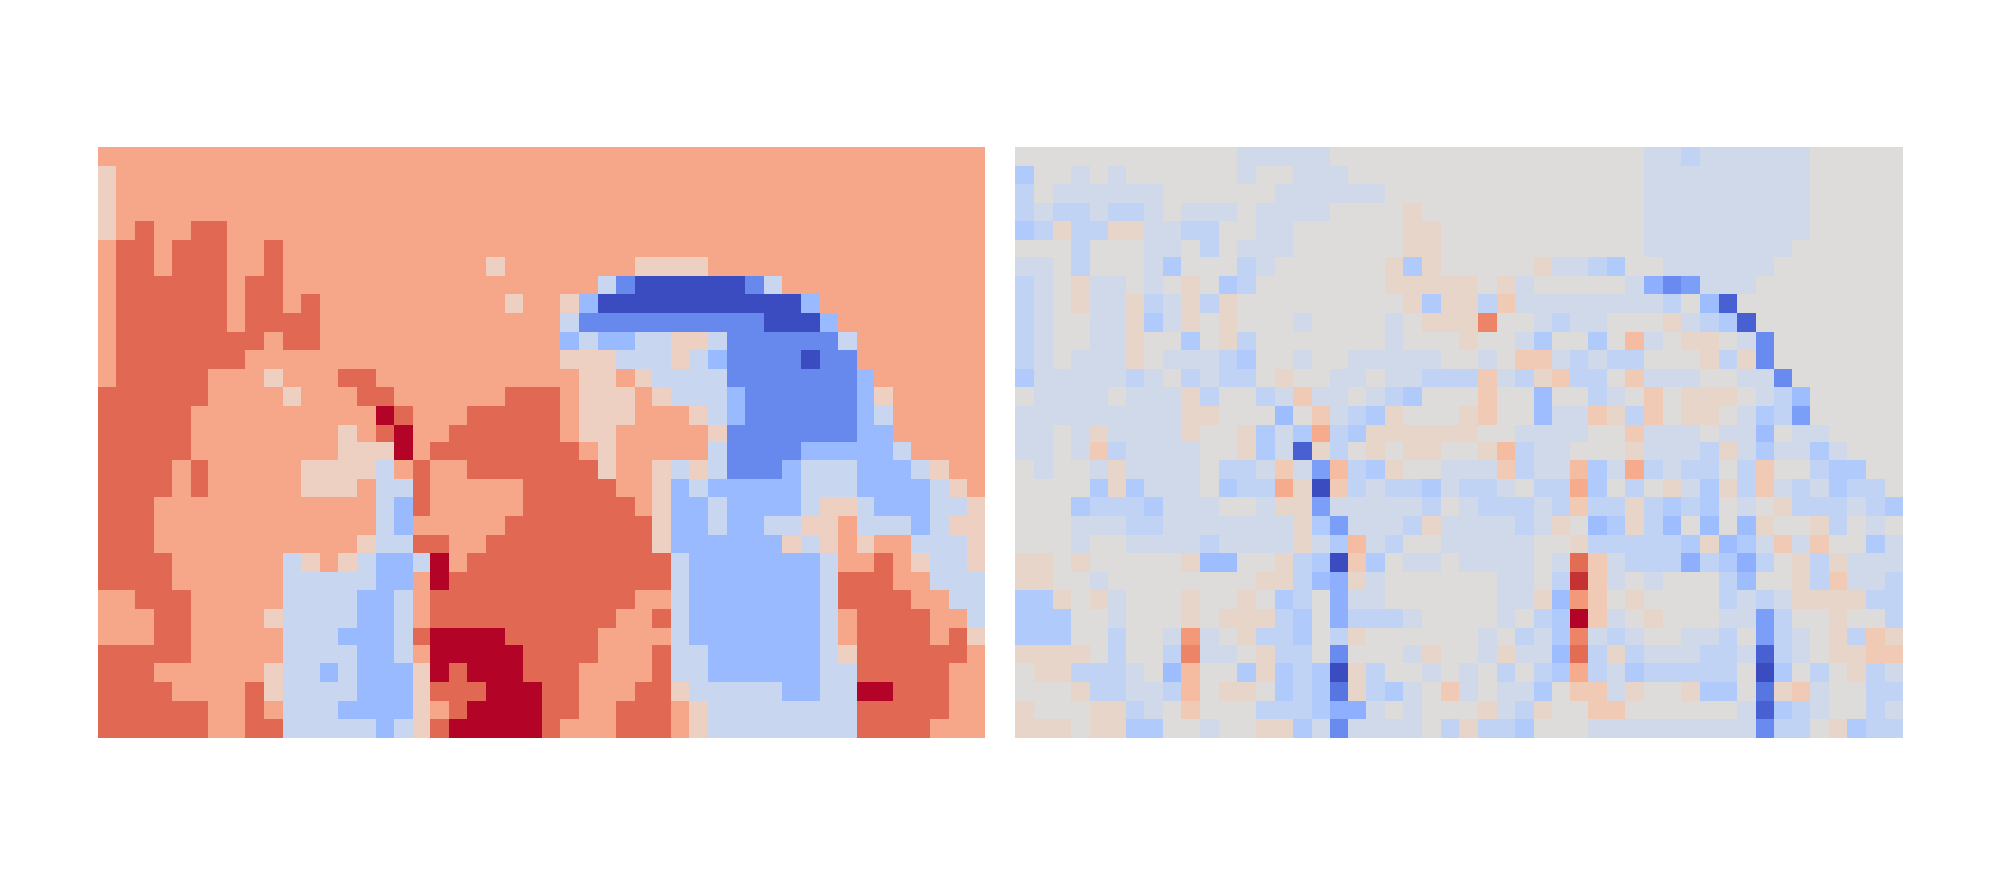
\includegraphics[width=.95\textwidth]{figures/kodim23_cr_components.pdf}
                \vspace{-15pt}
                \caption{$\bm{\mathcal{U}}_{C_R}$ channels}
            \end{subfigure}%
        \end{minipage}
    \end{minipage}
    \caption{The first channels of IMF factor maps for the \texttt{kodim23} image from Kodak, corresponding to luma ($Y$), blue-difference ($C_B$), and red-difference ($C_R$) chroma.}
	\label{fig:imf_components}
\end{figure}


\subsection{Decoding} \label{sec: decoding}

The decoder receives an encoded image and reconstructs the RGB image by applying the inverse of the operations used by the encoder, starting from the last layer and moving to the first. Initially, the factor maps defined in \eqref{eq: reshaped factors} are produced by losslessly decompressing the encoded image. These maps are then transformed into factor matrices by flattening their spatial dimensions. The matrices $\bm{X}_{Y}$, $\bm{X}_{C_B}$, and $\bm{X}_{C_R}$ are calculated through the product of the corresponding factor matrices due to \eqref{eq: lra}. The \emph{luma} and downsampled \emph{chroma} components are then obtained by reshaping $\bm{X}_{Y}$, $\bm{X}_{C_B}$, and $\bm{X}_{C_R}$ back into their spatial forms, following the inverse of the patchification step. Subsequently, the downsampled \emph{chroma} components are upsampled to their original size using bilinear interpolation. Finally, the YC\textsubscript{B}C\textsubscript{R} image is converted back into an RGB image. 

\subsection{Integer Matrix Factorization (IMF)} \label{sec: imf}

The main building block of our method is integer matrix factorization (IMF), which is responsible for the lossy compression of matrices obtained through patchification. IMF can be framed as an optimization problem, aiming to minimize the reconstruction error between the original matrix $\bm{X} \in \mathbb{R}^{M \times N}$ and the product $\bm{U} \bm{V}^\mathsf{T}$, while ensuring that the elements of the factor matrices $\bm{U}$ and $\bm{V}$ are integers within a specified interval $[\alpha,\beta]$ with integer values $\alpha$ and $\beta$, i.e., $\alpha,\beta\in\Z$. Formally, the IMF problem can be expressed as:
\begin{align} \label{eq: imf problem}
	\minimize_{\bm{U}, \bm{V}} & \ \  \| \bm{X} - \bm{U} \bm{V}^\mathsf{T} \|_\text{F}^2 \nonumber \\
	\text{s.t.}           & \ \ \bm{U} \in \mathbb{Z}_{[\alpha,\beta]}^{M \times R}, \bm{V} \in \mathbb{Z}_{[\alpha,\beta]}^{N \times R},
\end{align}
where $\|\cdot\|_\text{F}$ denotes the Frobenius norm; $R \leq \min(M,N)$ represents the \emph{rank}; and $\mathbb{Z}_{[\alpha,\beta]} \triangleq [\alpha,\beta] \cap \mathbb{Z}$ denotes the set of integers within $[\alpha,\beta]$. Without constraints on the factors, the problem would have an analytic solution through the singular value decomposition (SVD), as addressed by the Eckart–Young–Mirsky theorem \cite{eckart1936approximation}. If only a nonnegativity constraint were applied (without integrality), variations of nonnegative matrix factorization (NMF) would emerge \cite{lee2000algorithms, gillis2020nonnegative}. The IMF problem \eqref{eq: imf problem} poses a challenging integer program, with finding its global minima known to be NP-hard \cite{dong2018integer, van1981another}. Only a few iterative algorithms \cite{dong2018integer, lin2005integer} have been proposed to find a ``good solution'' for some IMF variants in contexts other than image compression. In Section \ref{sec: bcd}, we propose an efficient iterative algorithm for the IMF problem \eqref{eq: imf problem}.

The application of SVD and NMF in image compression is problematic mainly because the resulting factors contain continuous values that must be represented as arrays of floating-point numbers. This necessitates a quantization step that not only adds extra complications but also significantly degrades compression performance due to quantization errors (as demonstrated in Section \ref{sec: experiments}). Conversely, our IMF formulation produces integer factor matrices that can be directly stored and losslessly processed without incurring roundoff errors. The reason for limiting the feasible region to $[\alpha,\beta]$ in our IMF formulation is to enable more compact storage of the factors using standard integral data types, such as \texttt{int8} and \texttt{int16}, supported by programming languages. Given that the elements of the input matrix $\bm{X}$ are in $[0, 255]$, we found the signed \texttt{int8} type, which represents integers from -128 to 127, suitable for image compression applications. As a result, our IMF formulation is well-suited for image compression, effectively integrating the factorization and quantization steps into a single, efficient compression process.


\subsection{Block Coordinate Descent Scheme for IMF} \label{sec: bcd}

\begin{algorithm}[!t]
	\caption{The proposed block coordinate descent (BCD) algorithm for IMF. \label{alg: bcd for imf}}
	\DontPrintSemicolon
	\SetAlgoLined
	\KwIn{$\bm{X} \in \mathbb{R}^{M \times N}$, factorization rank $R$}
	\KwOut{Factor matrices $\bm{U} \in \mathbb{Z}_{[\alpha,\beta]}^{M \times R}$ and $\bm{V} \in \mathbb{Z}_{[\alpha,\beta]}^{N \times R}$}
	Initialize $\bm{U}^{\rm init}$, $\bm{V}^{\rm init}$ using the truncated SVD method, provided by \eqref{eq: initialization: u} and \eqref{eq: initialization: v}, and set $k=0$\;
	\While{stopping criterion not satisfied}{
        $k \gets k+1$\;
		$\bm{A} \gets \bm{X} \bm{V}^k$,\ $\bm{B} \gets \bm{V}^{k^{\mathsf{T}}} \bm{V}^k$\;
		\For{$r = 1, \ldots, R$}{
			$\displaystyle U_{:r}^{k+1} = \round \Big(\clamp_{[\alpha,\beta]}\Big(\frac{A_{:r} - \sum_{s = 1}^{r-1} B_{sr} U_{:s}^{k+1} - \sum_{s=r+1}^M B_{sr} U_{:s}^k}{\| V_{:r}^k \|^2}\Big)\Big)$\;
		}
		$\bm{A} \gets \bm{X}^\mathsf{T} \bm{U}^{k+1}$; $\bm{B} \gets \bm{U}^{{k+1}^\mathsf{T}} \bm{U}^{k+1}$\;
		\For{$r = 1, \ldots, R$}{
			$\displaystyle V_{:r}^{k+1} = \round \Big(\clamp_{[\alpha,\beta]}\Big(\frac{A_{:r} - \sum_{s = 1}^{r-1} B_{sr} V_{:s}^{k+1} - \sum_{s = r+1}^N B_{sr} V_{:s}^k}{\| U_{:r}^{k+1} \|^2}\Big)\Big)$\;
		}
	}
	\Return $(\bm{U}^k, \bm{V}^k)$
\end{algorithm}

We propose an efficient algorithm for IMF using the block coordinate descent (BCD) scheme (aka alternating optimization). 
The pseudocode is provided in Algorithm \ref{alg: bcd for imf}.
Starting with some initial parameter values, this approach involves sequentially minimizing the cost function with respect to a single column of a factor at a time, while keeping the other columns of that factor and the entire other factor fixed. This process is repeated until a stopping criterion is met, such as when the change in the cost function value falls below a predefined threshold or the maximum number of iterations is reached. Formally, this involves solving one of the following subproblems at a time:
\begin{align}  
	\bm{u}_r \gets \underset{\bm{u}_r \in \mathbb{Z}_{[\alpha,\beta]}^M}{\argmin} \ \lVert \bm{E}_r - \bm{u}_r \bm{v}_r^\mathsf{T} \rVert_\text{F}^2, \label{eq: bcd subproblem: u} \\
	\bm{v}_r \gets \underset{\bm{v}_r \in \mathbb{Z}_{[\alpha,\beta]}^N}{\argmin} \ \lVert \bm{E}_r - \bm{u}_r \bm{v}_r^\mathsf{T} \rVert_\text{F}^2, \label{eq: bcd subproblem: v}
\end{align}
where $\bm{u}_r \coloneqq U_{:r}$ and $\bm{v}_r \coloneqq V_{:r}$ represent the $r$-th columns of $\bm{U}$ and $\bm{V}$, respectively. $\bm{E}_r \coloneqq \bm{X} - \sum_{s \neq r}^{R} \bm{u}_s \bm{v}_s^\mathsf{T}$ is the residual matrix. We define one iteration of BCD as a complete cycle of updates across all the columns of both factors. In fact, the proposed algorithm is a $2R$-block coordinate descent procedure, where at each iteration, first the columns of $\bm{U}$ and then the columns of $\bm{V}$ are updated (see Algorithm \ref{alg: bcd for imf}). Note that subproblem \eqref{eq: bcd subproblem: v} can be transformed into the same form as \eqref{eq: bcd subproblem: u} by simply transposing its error term inside the Frobenius norm. Therefore, we only need to find the best rank-1 approximation with integer elements constrained within a specific interval. Fortunately, this problem has a closed-form solution, as addressed by Theorem \ref{the: bcd subproblem} below.
\bigskip
\begin{theorem}[Integer rank-1 approximation] \label{the: bcd subproblem}
    The global optima of subproblems \eqref{eq: bcd subproblem: u} and \eqref{eq: bcd subproblem: v} can be represented by closed-form solutions. Specifically, these subproblems can be replaced by the following:
    \begin{align} 
            \textstyle \bm{u}_r \gets \round\big(\clamp_{[\alpha,\beta]}\big(\frac{\bm{E}_r \bm{v}_r}{\lVert \bm{v}_r \rVert^2}\big)\big), \label{eq:bcd_closed_form_subproblem_u}\\
            \textstyle \bm{v}_r \gets \round\big(\clamp_{[\alpha,\beta]}\big(\frac{\bm{E}_r^\mathsf{T} \bm{u}_r}{\lVert \bm{u}_r \rVert^2}\big)\big),             
        \label{eq:bcd_closed_form_subproblem_v}
    \end{align}
    where $\round(\bm{Z})$ denotes an element-wise operator that rounds each element of $\bm{Z}$ to the nearest integer, and $\clamp_{[\alpha,\beta]}(\bm{Z}) \triangleq \max(\alpha, \min(\bm{Z}, \beta))$ denotes an element-wise operator that clamps each element of $\bm{Z}$ to the interval $[\alpha,\beta]$.
\end{theorem}
\begin{proof}
	See Appendix \ref{app: proof:1} for the proof.
\end{proof}

It is noteworthy that the combination of $\round(\cdot)$ and $\clamp_{[\alpha,\beta]}(\cdot)$ in \eqref{eq:bcd_closed_form_subproblem_u} and \eqref{eq:bcd_closed_form_subproblem_v} can be interpreted as the element-wise projector to $\mathbb{Z}_{[\alpha,\beta]}$. In Theorem \ref{thm:convergence}, the convergence of the proposed algorithm employing these closed-form solutions will be established.
\bigskip
\begin{theorem}[Global convergence]\label{thm:convergence}
    Let $\seq{\bm U^k}[k\in\N]$ and $\seq{\bm V^k}[k\in\N]$ be sequences generated by the proposed Algorithm \ref{alg: bcd for imf}. Then both sequences are convergent to a locally optimal point of the optimization problem \eqref{eq: imf problem}.
\end{theorem}
\begin{proof}
    See Appendix \ref{app: proof:2} for the proof.
\end{proof}




% \begin{theorem}[Integer rank-1 approximation] \label{the: bcd subproblem}
% 	Let $\bm{E} \in \mathbb{R}^{M \times N}$, $\bm{u} \in \mathbb{Z}_{[\alpha,\beta]}^{M \times 1}$, and $\bm{v} \in \mathbb{R}^{N \times 1}$. A global solution to the problem
% 	\begin{equation} \label{eq: bcd subproblem}
% 		\bm{u}^* \in \underset{\bm{u} \in \mathbb{Z}_{[\alpha,\beta]}^{M \times 1}}{\argmin} \ \lVert \bm{E} - \bm{u} \bm{v}^\mathsf{T} \rVert_\text{F}^2
% 	\end{equation}
% 	is given by
% 	\begin{equation} \label{eq: bcd subproblem solution}
% 		\bm{u}^* = \clamp_{[\alpha,\beta]}\Big(\round\Big(\frac{\bm{E} \bm{v}}{\lVert \bm{v} \rVert^2}\Big)\Big),
% 	\end{equation} 
% 	where $\round(\bm{Z})$ denotes the operator that rounds each element of $\bm{Z}$ to the nearest integer, and $\clamp_{[\alpha,\beta]}(\bm{Z}) \triangleq \max(\alpha, \min(\bm{Z}, \beta))$ denotes the operator that clamps each element of $\bm{Z}$ to the interval $[\alpha,\beta]$.
% \end{theorem}

% Using Theorem \ref{the: bcd subproblem}, we obtain the following update formulas for our BCD algorithm:
% Thanks to Theorem \ref{the: bcd subproblem}, the proposed algorithm offers an encouraging property that guarantees the cost function is monotonically non-increasing with each update. 


\paragraph{Initialization.}
The initial values of factors can significantly impact the convergence performance of the BCD algorithm. We found that the convergence with naive random initialization can be too slow. To address this issue, we propose an initialization method using SVD. The procedure is straightforward. First, the truncated SVD of the input matrix $\bm{X} \in \mathbb{R}^{M \times N}$ is computed as $\tilde{\bm{U}} \bm{\Sigma} \tilde{\bm{V}}^\mathsf{T}$, where $\bm{\Sigma} \in \mathbb{R}^{R \times R}$ is a diagonal matrix corresponding to the $R$ largest singular values. $\tilde{\bm{U}} \in \mathbb{R}^{M \times R}$ contains the corresponding left-singular vectors in its columns, and $\tilde{\bm{V}} \in \mathbb{R}^{N \times R}$ contains the corresponding right-singular vectors in its columns. The initial factors are then calculated as follows:
\begin{align} 
	\bm{U}^{\rm init} = \round(\clamp_{[\alpha,\beta]}(\tilde{\bm{U}} \bm{\Sigma}^\frac{1}{2})), \label{eq: initialization: u} \\
	\bm{V}^{\rm init} = \round(\clamp_{[\alpha,\beta]}(\bm{\Sigma}^\frac{1}{2} \tilde{\bm{V}})). \label{eq: initialization: v}
\end{align}
Essentially, this means we first low-rank approximate $\bm{X}$ and then project the elements of the resulting factor matrices into $\mathbb{Z}_{[\alpha,\beta]}$. 

